\documentclass[12pt]{article}
\usepackage[top=1in, bottom=1in, left=.75in, right=.75in]{geometry}
\usepackage{amsmath}
\usepackage{fancyhdr}
\usepackage{graphicx}
\usepackage{txfonts}
\usepackage{multicol,coordsys}
\usepackage[scaled=0.86]{helvet}
\renewcommand{\emph}[1]{\textsf{\textbf{#1}}}
\usepackage{anyfontsize}
% \usepackage{times}
% \usepackage[lf]{MinionPro}
\usepackage{tikz,pgfplots}
%\def\degC{{}^\circ{\rm C}}
\def\ra{\rightarrow}
\usetikzlibrary{calc}
\pgfplotsset{compat = newest}
\newcommand{\blank}[1]{\rule{#1}{0.75pt}}

\pgfplotsset{my style/.append style={axis x line=middle, axis y line=
middle, xlabel={$x$}, ylabel={$y$},axis equal}}

%yticklabels={,,} , xticklabels={,,}

% \setmainfont{Times}
% \def\sansfont{Lucida Grande Bold}
\parindent 0pt
\parskip 4pt
\pagestyle{fancy}
\fancyfoot[C]{\emph{\thepage}}
\fancyhead[L]{\ifnum \value{page} > 1\relax\emph{Math 251: Midterm 1}\fi}
\fancyhead[R]{\ifnum \value{page} > 1\relax\emph{February 10, 2022}\fi}
\headheight 15pt
\renewcommand{\headrulewidth}{0pt}
\renewcommand{\footrulewidth}{0pt}
\let\ds\displaystyle
\def\continued{{\emph {Continued....}}}
\def\continuing{{\emph {Problem \arabic{probcount} continued....}}\par\vskip 4pt}


\newcounter{probcount}
\newcounter{subprobcount}
\newcommand{\thesubproblem}{\emph{\alph{subprobcount}.}}
\def\problem#1{\setcounter{subprobcount}{0}%
\addtocounter{probcount}{1}{\emph{\arabic{probcount}.\hskip 1em(#1)}}\par}
\def\subproblem#1{\par\hangindent=1em\hangafter=0{%
\addtocounter{subprobcount}{1}\thesubproblem\emph{#1}\hskip 1em}}
\def\probskip{\vskip 10pt}
\def\medprobskip{\vskip 2in}
\def\subprobskip{\vskip 45pt}
\def\bigprobskip{\vskip 4in}

\begin{document}
{\emph{\fontsize{26}{28}\selectfont Math F251\hfill
{\fontsize{32}{36}\selectfont Midterm 1}
\hfill Spring 2022}}
\vskip 2cm
\strut\vtop{\halign{\emph#\hskip 0.5em\hfil&#\hbox to 2in{\hrulefill}\cr
\emph{\fontsize{18}{22}\selectfont Name:}&\cr
\noalign{\vskip 10pt}
%\emph{\fontsize{18}{22}\selectfont Student Id:}&\cr
%\noalign{\vskip 10pt}
%\emph{\fontsize{18}{22}\selectfont Calculator Model:}&\cr
}}
\hfill
\vtop{\halign{\emph{\fontsize{18}{22}\selectfont #}\hfil& \emph{\fontsize{18}{22}\selectfont\hskip 0.5ex $\square$ #}\hfil\cr
Section: & F01 (Jill Faudree)\cr
\noalign{\vskip 4pt}
         & F02 (James Gossell)\cr
\noalign{\vskip 4pt}
         & UX1 (James Gossell)\cr}}

\vfill
{\fontsize{18}{22}\selectfont\emph{Rules:}}

You have 60 minutes to complete the exam.  

Partial credit will be awarded, but you must show your work.

The exam is closed book and closed notes.

Calculators are not allowed. 


Place a box around your  \fbox{FINAL ANSWER} to each question where appropriate.

%If you need extra space, you can use the back sides of the pages.
%Please make it obvious  when you have done so.

Turn off anything that might go beep during the exam.

Good luck!
\vfill
\def\emptybox{\hbox to 2em{\vrule height 16pt depth 8pt width 0pt\hfil}}
\def\tline{\noalign{\hrule}}
\centerline{\vbox{\offinterlineskip
{
\bf\sf\fontsize{18pt}{22pt}\selectfont
\hrule
\halign{
\vrule#&\strut\quad\hfil#\hfil\quad&\vrule#&\quad\hfil#\hfil\quad
&\vrule#&\quad\hfil#\hfil\quad&\vrule#\cr
height 3pt&\omit&&\omit&&\omit&\cr
&Problem&&Possible&&Score&\cr\tline
height 3pt&\omit&&\omit&&\omit&\cr
&1&&12&&\emptybox&\cr\tline
&2&&20&&\emptybox&\cr\tline
&3&&10&&\emptybox&\cr\tline
&4&&8&&\emptybox&\cr\tline
&5&&6&&\emptybox&\cr\tline
&6&&8&&\emptybox&\cr\tline
&7&&8&&\emptybox&\cr\tline
&8&&15&&\emptybox&\cr\tline
&9&&15&&\emptybox&\cr\tline
&Extra Credit&&5&&\emptybox&\cr\tline
&Total&&100&&\emptybox&\cr
}\hrule}}}

\newpage
\begin{enumerate}
%%%PAGE 1
%%%%LIMITS + DERIVATIVES FROM GRAPHs
\item{(12 points)} Use the graph of the function $f(x)$, sketched below, to answer the questions. The dotted line at $x=4$ represents a vertical asymptote. You must give the most complete answer; if an answer is $\infty$ or $-\infty$, you must indicate this. 

%%%%FIGURE
\begin{center}
 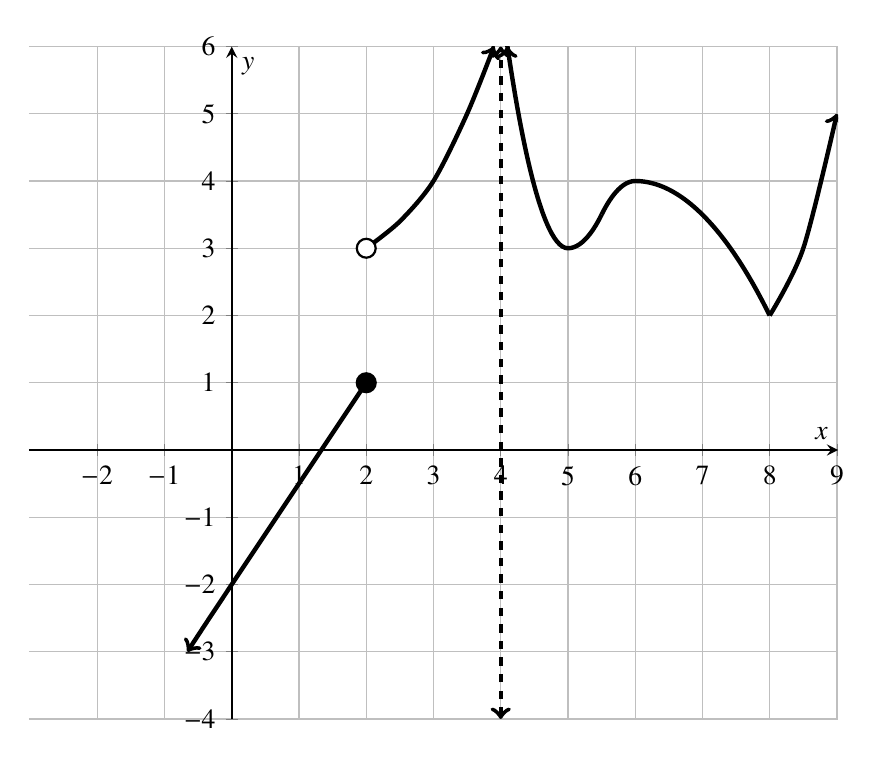
\begin{tikzpicture}
\begin{axis}[x=1cm,y=1cm,scale=1.5,xscale=1, thick, my style, xtick={-2,-1,...,8,9}, ytick={-4,-3,...,6},xmin=-2, xmax=8, ymin=-4, ymax=6, 
mark size=3.0pt, grid = major]
\addplot[smooth,ultra thick,<-] coordinates {(-0.66,-3) (0,-2) (2,1)};
\addplot[smooth,ultra thick,->] coordinates {(2,3) (2.5,3.4) (3,4) (3.5,5) (3.9,6) };
\addplot[ultra thick,<-] (4.1,6) parabola bend (5,3)  (5.5,3.5);
\addplot[ultra thick,] (5.5,3.5) parabola bend (6,4)  (8,2);
\addplot[smooth,ultra thick,->] coordinates {(8,2) (8.5,3) (9,5)  };
%\node at (-2.5,2.5){\large{$f(x)$}};
\draw[fill=white, thick] (2,3) circle  (1.2 mm);
\draw[fill=black, thick] (2,1) circle  (1.2 mm);
\addplot[ultra thick, <->, dashed] coordinates{(4,-4)(4,6)};
\end{axis}
\end{tikzpicture}\end{center}

\newcommand{\ans}{\rule{1.5cm}{.5 pt}}
\newlength{\mysep} 
\setlength{\mysep}{0.3in}
%%%%%QUESTIONS
\begin{enumerate}
\begin{multicols}{2}
\item $\displaystyle{\lim_{x\to 2^{-}} f(x) }= \ans$
\bigskip

\item $ \displaystyle{ \lim_{x\to 2^+} f(x) }= \ans$
\bigskip

\item $ \displaystyle{ \lim_{x\to 2} f(x) }= \ans$
\bigskip

\item $f(2) = \ans$
\bigskip

\item $\displaystyle{ \lim_{x \to 4} f(x) }= \ans$
\bigskip

\item $\displaystyle{ \lim_{x \to 8^+} f(x) }= \ans$
\bigskip

\item $ \large{f'(1)}= \: \ans $
\bigskip

\item $ \large{f'(5)}= \: \ans $
\bigskip


\vspace{\mysep}
\end{multicols}
\vspace{1cm}
\item List the $x$-values where $f(x)$ fails to be continuous.\\
\vfill
\item List the $x$-values for which $f(x)$ fails to have a derivative.\\\vfill
\vspace{\mysep}
\end{enumerate}
\newpage
%%%%%%%PAGE 2
%%%%%%%ASSORTMENT OF LIMITS
\item (20 points)  Evaluate the following limits. Give the most complete answer; if the limit is infinite, indicate that with $\infty$ or $-\infty.$ If a value does not exist, write DNE.\\
	\begin{enumerate}
	\item $\displaystyle{\lim_{x \to 1 } \frac{x^2+2x-3}{2x^2-x-1} =}$
	\vfill
	\item $\displaystyle{\lim_{x \to 2^+ }  \frac{x-\sqrt{2+x}}{x^2+4}=}$
	\vfill
	\item $\displaystyle{\lim_{x \to -4} \left(\frac{\frac{1}{4} + \frac{1}{x}}{x+4} \right)=}$
	\vfill
	\item $\displaystyle{\lim_{x  \to 10^+} \frac{1-4x}{(10-x)^3}=}$
	\vfill
	
	
	\end{enumerate}
\newpage

%%%%PAGE 3
%%%%%DEFINTION OF DERIVATIVE
\item (10 points) Find the derivative of $f(x) = x^2 + 4x$  using the limit definition of the derivative $$f'(x)=\displaystyle{\lim_{h \rightarrow 0}\frac{f(x+h)-f(x)}{h}}.$$ No credit will be awarded for using other methods.
\newpage
%%%%PAGE 3
%continuity
\item (8 points) Is the following function continuous at $x=3$? Justify your answer. 

$
f(x) = \begin{cases}
\frac{6-2x}{x-3} & \text{if } x \leq 3\\
2  & \text{if } x =3\\
x-5  & \text{if } x \geq 3
\end{cases}
$

\vfill

%\item (5 points) NEW Sketch a graph of a function that has a \textbf{removable} disconinuity at $x=-2$  and a \textbf{non removable} discontinuity at $x=2$.
%        \begin{center}
%        \rescaleby{1}{11}{\vlabel}
%        \rescaleby{1}{11}{\hlabel}
%        \coordsys[11][11](-110,-110)(110,110)
%        \end{center}
%
%\vspace{0.5in}

\item (6 points) Does the function $g(x)=4\sin x - 5\cos x$ pass through the x-axis on the interval $[0,\frac{\pi}{2}]$? Justify your answer. (Hint: Use the Intermediate Value Theorem.)

\vfill
\newpage


%%%%%%%%APPLIED EXPLANATION
\item (8 points) Let $H(t)$ be the daily cost, in dollars, of heating a building when the outside temperature is $t$ degrees Fahrenheit.

	\begin{enumerate}

	\item What is the meaning of $H(0)=50$? Your answer should be a complete sentence and must include units.

	\vspace{.6in}

	\item What are the units of $H'(t)$?
	\vspace{.5in}

	\item Do you expect $H'(t)$ to be positive or negative? \textbf{Justify} your answer using complete sentences. 
\vfill
	\end{enumerate}


%%%%SKETCH DERIVATIVE FROM GRAPH OF FUNCTION
\item (8 points) The graph of $g(x)$ is graphed below. On the same set of axes, sketch the graph of its derivative $g'(x)$.

\begin{center}
 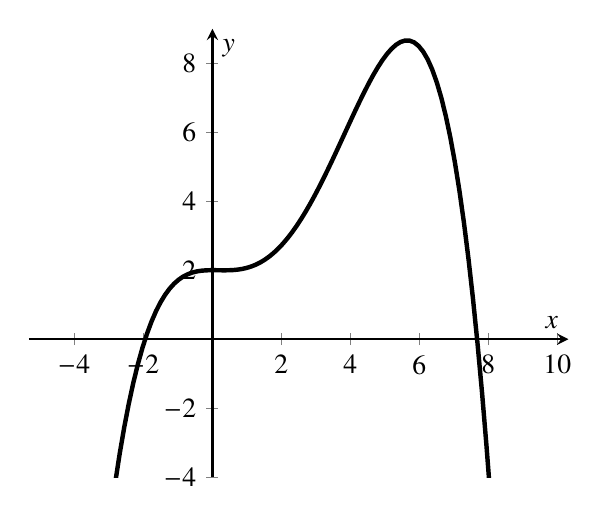
\begin{tikzpicture}
\begin{axis}[scale=1,xscale=1, thick, my style,xmin=-4, xmax=9, ymin=-4, ymax=9, 
mark size=3.0pt, ]
\addplot[ultra thick, ->,domain=-4:9, samples=100]{-1*((0.09)*(0.25*x*x*x*x-2*x*x*x+x*x))+2};
%\addplot[ultra thick, <-,domain=-6:0, samples=100]{-x};
%\node at (10,2){$g(x)$};
\end{axis}
\end{tikzpicture}\end{center}

\newpage

%%%%PAGE 5
%%%%%%%% STRAIGHT DERIVATIVES
\item (15 points) Find $f'(x)$ for each of the following expressions. You do not need to simplify.

	\begin{enumerate}
	\item $f(x) = 3\cos x + 2x^3 - \frac{1}{x^2}+\sqrt{5}$
        \vfill
%    \item $f(x) = \frac{2x^2-4x+1}{\sqrt{x}}$
%        \vfill
       
    \item $f(x)=\frac{\sin x}{x^3-1}$
        \vfill
        \item $f(x)= x^{2.3} + x \cos(x)$
       \vfill
	\end{enumerate}
\newpage
\item (15 points) The mars rover launches a sensor vertically upward from an arm 1 meter above the surface of the planet. The height, in meters, of the sensor $t$ seconds after launch is given by $$h(t)=1+8t-2t^2.$$ {\bf Include units in your answers}.

	\begin{enumerate}
	\item Find the velocity function and the acceleration function for the sensor.\\
	\vfill

	\item What is the initial velocity of the sensor?\\ \vfill

	\item What is the average velocity of the sensor in the interval from $t=1$ to $t=4$?\\ \vfill

	%\item How high will the football go?\\ \vfill

	\item Four seconds after launch (when $t=4$) is the sensor speeding up or slowing down? Justify your answer.\\ \vfill

	\item What is the acceleration due to gravity on mars?\\ \vspace{.5in}

\end{enumerate}
\newpage
\item \textbf{Extra Credit} (5 points) Find $\frac{d}{dx}\left(\sec x\right)$ by rewriting $\sec x$ as $\frac{1}{\cos x}$ and using the quotient rule. For full credit, please simplify your final answer.

\vfill
\end{enumerate}
\end{document}













